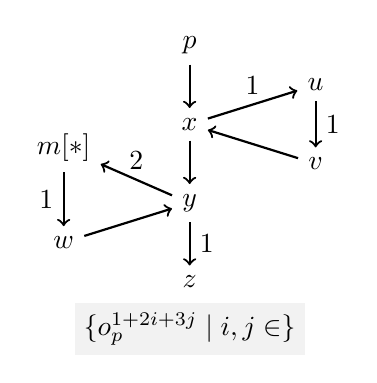
\begin{tikzpicture}[scale=1,thick]
    \node (p) at (0, 0) {$\textpurple{p}$};
    \node (x) at (0, -1) {$x$};
    \node (u) at (1.6, -0.5) {$u$};
    \node (v) at (1.6, -1.5) {$v$};
    \node (y) at (0, -2) {$y$};
    \node (m) at (-1.6, -1.3) {$m[*]$};
    \node (w) at (-1.6, -2.5) {$w$};



    \node (z) at (0, -3) {$z$};
    \node[fill=gray!10] at (0, -3.6) {$\{o_p^{1 + 2i + 3j} \mid  i, j \in \nats\}$};

    \draw [->] (p) -- (x);
    \draw [->] (x) --node[above]{$1$} (u);
    \draw [->] (u) --node[right]{$1$} (v);
    \draw [->] (v) -- (x);
    \draw [->] (x) -- (y);
    \draw [->] (y) --node[above]{$2$} (m);
    \draw [->] (m) --node[left]{$1$} (w);
    \draw [->] (w) -- (y);
    \draw [->] (y) --node[right]{$1$} (z);
\end{tikzpicture}
